\documentclass[11pt]{preprint}

\setlength{\topmargin}{0mm} \setlength{\oddsidemargin}{0mm}
\setlength{\textwidth}{160mm} \setlength{\textheight}{215mm}

\usepackage{amssymb,amsmath,amscd,amsthm}
\usepackage{tikz}
\usepackage{wrapfig}

\newtheorem{proposition}{Proposition}

\def\enumb{\begin{enumerate}}
\def\enume{\end{enumerate}}
\def\integers{\mathbb{Z}}
\def\multiset#1#2{\ensuremath{\left(\kern-.3em\left(\genfrac{}{}{0pt}{}{#1}{#2}\right)\kern-.3em\right)}}

\title{Discrete Mathematics, 2016 Fall - HW 13 (Optional)}
\author{Instructor: Zsolt Pajor-Gyulai}
\institute{Courant Institute of Mathematical Sciences, NYU}



\begin{document}

\maketitle

To get full credit  in all of the problems, use rigorous justification and unless otherwise indicated, make sure that your solution reads as a perfect English sentence. You should only assume integers, operations and order relations as given. If you use a statement or a definition from the textbook, make sure to indicate it.
\vspace{0.2cm}


\textbf{Section 49}
\enumb
\item[4)] Let $n\geq 2$ be an integer. Form a graph $G_n$ whose vertices are all the two-element subsets of $\{1,2,\dots,n\}$. In this graph, we have an edge between distinct vertices $\{a,b\}$ and $\{c,d\}$ exactly when $\{a,b\}\cap\{c,d\}=\emptyset$.
\enumb
\item How many vertices does $G_n$ have?
\item How many edges does $G_n$ have?
\item For which values of $n\geq 2$ is $G_n$ connected? Prove your answer.
\enume
\item[6)] Let $G$ be a graph. A path $P$ in $G$ that contains all the vertices of $G$ is called a \textbf{Hamiltonian path}. Prove that the following graph does not have a Hamiltonian path. 

\begin{figure}[ht]
\centering
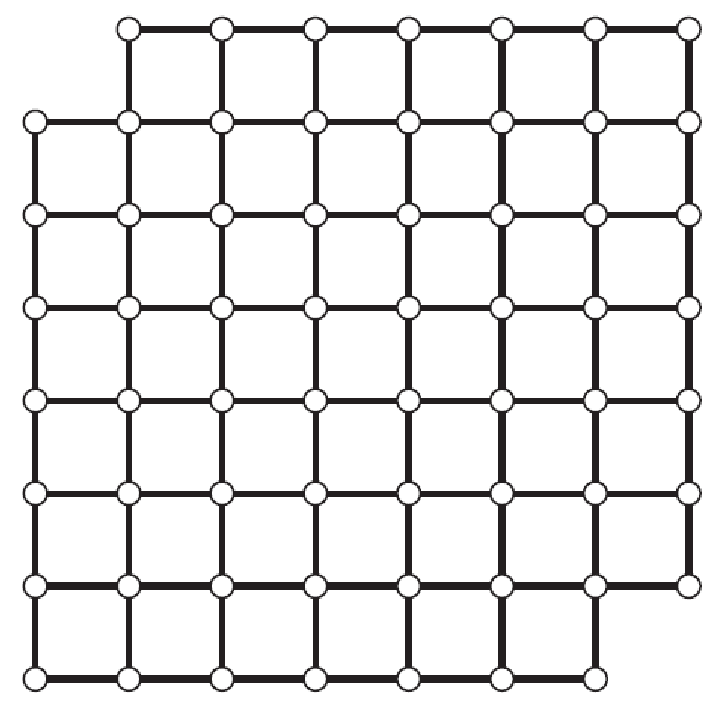
\includegraphics[scale=0.3]{HW1.pdf}
\end{figure}
\item[10)] Let $G$ be a graph. Prove that $G$ or $\bar{G}$ or both must be connected.
\enume

\textbf{Section 50}
 \enumb
\item[5)] Let $e$ be an edge of a graph $G$. Prove that $e$ is not a cut edge if and only if $e$ is in a cylce of $G$.
\item[10)] Prove that a graph is a forest if and only if all of its edges are cut edges.
\item[16)] Let $G$ be a graph. A cycle of $G$ that contains all the vertices in $G$ is called a \textbf{Hamiltonian cycle}.
\enumb
\item Show that $n\geq 5$, then $\bar{C}_n$ has a Hamiltonian cycle.
\item Prove that the graph in the figure does not have a Hamiltonian cycle.
\enume
\begin{figure}[ht]
\centering
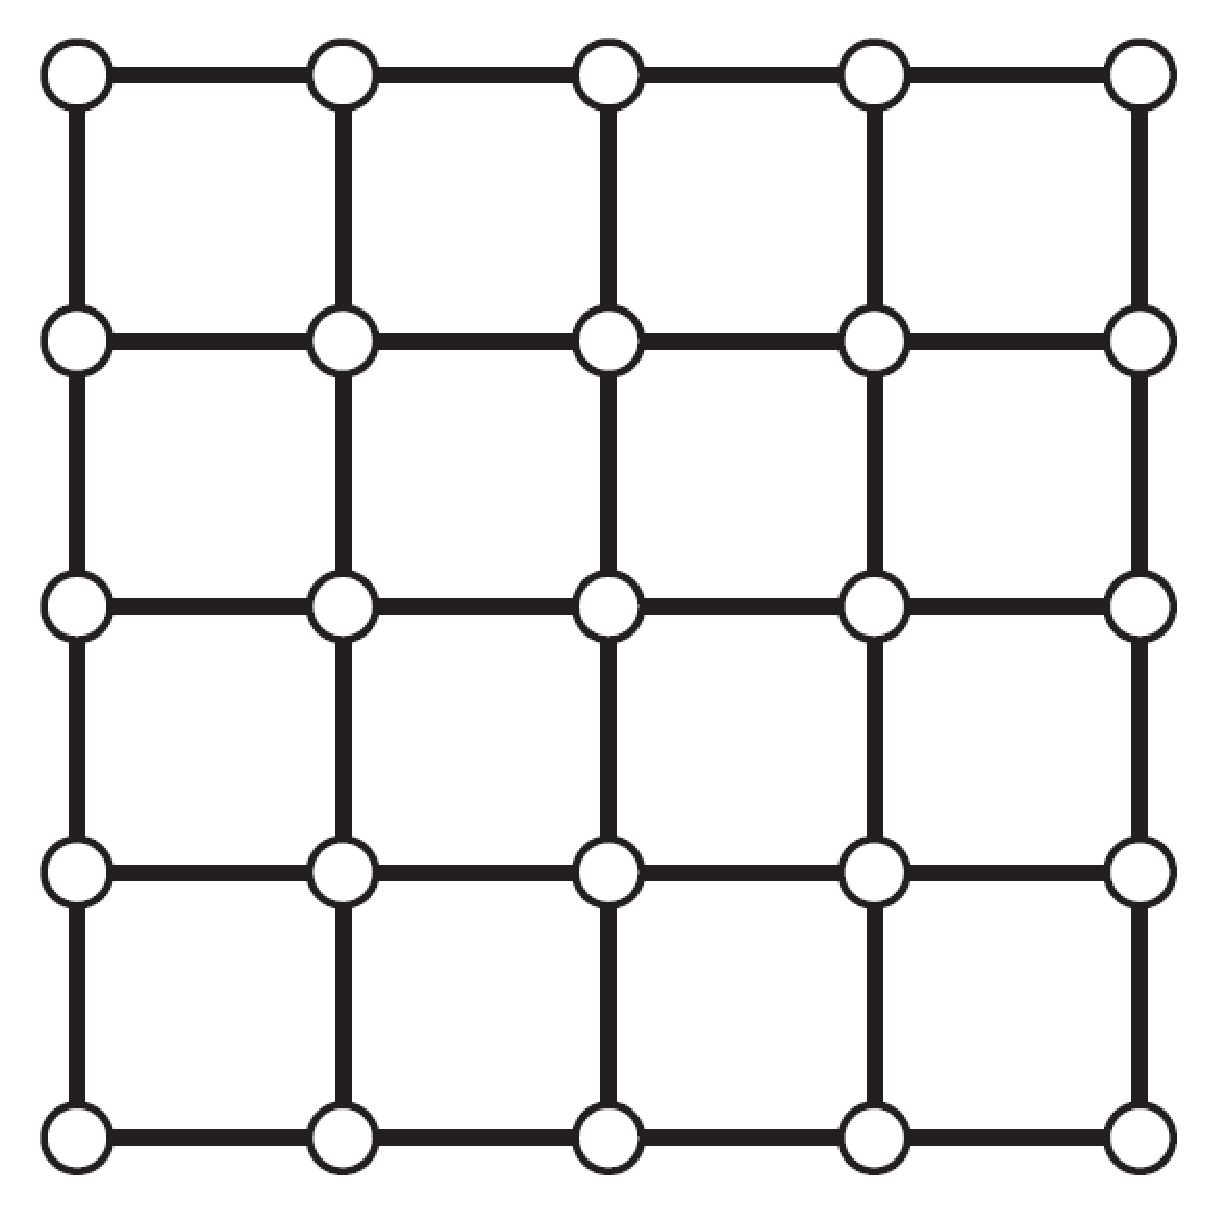
\includegraphics[scale=0.22]{HamltonCirc.pdf}
\end{figure}
\enume

\textbf{Section 51}

\enumb
\item [6)] Let $G$ be an Eulerian graph. Prove that it is possible to partition the edge set of $G$ such that the edges in each part of the partition form a cycle of $G$.
\item [7)] A rook is a chess piece that may, on a single turn, move any number of squares horizontally or any number of squares vertically on the board. That is, if squares $A$ and $B$ are in the same row [or same column] then we are permitted to move the rook from $A$ to $B$. Other moves, however, are illegal. Thus in every row and every column there are $\binom{8}{2}$ pairs of squares between which the rook may move. This gives a total of $16\binom{8}{2}=448$ such pairs.

Suppose a rook is placed on an empty chess board. Can we repeatedly move the rook so that it moves exactly once between each pair of squares in the same row and once between each pair of squares in the same column?
\enume
\textbf{Section 52}

\enumb
\item[1)] Let $H$ be the graph in the following figure.
\begin{figure}[ht]
\centering
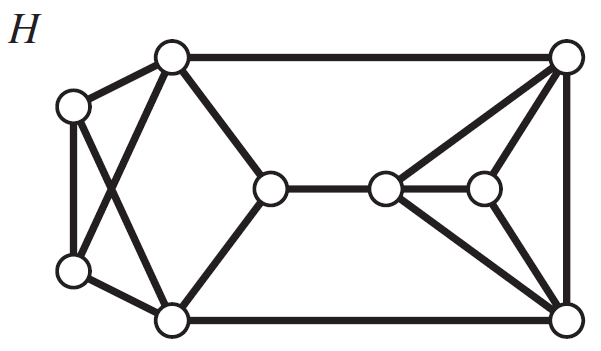
\includegraphics[scale=0.4]{Color1.jpg}
\end{figure}
Please find $\chi(H)$.
\item[8)] Let $G$ be a graph with $n$ vertices. Prove that $\chi(G)\geq\omega(G)$ and $\chi(G)\geq n/\alpha(G)$.
\item[14)] Suppose $G$ has maximum degree $\Delta>1$, but it has only one vertex of degree $\Delta$. Prove that $\chi(G)\leq\Delta$.
\enume

\end{document}